\section{Kombinatorische Logik}

\subsection{Logische Gatter}

\subsubsection{NOT} 
\begin{center}
    \begin{minipage}{0.55\linewidth}
		$Y \neq A$ \\
		Y != A
        \begin{center}
		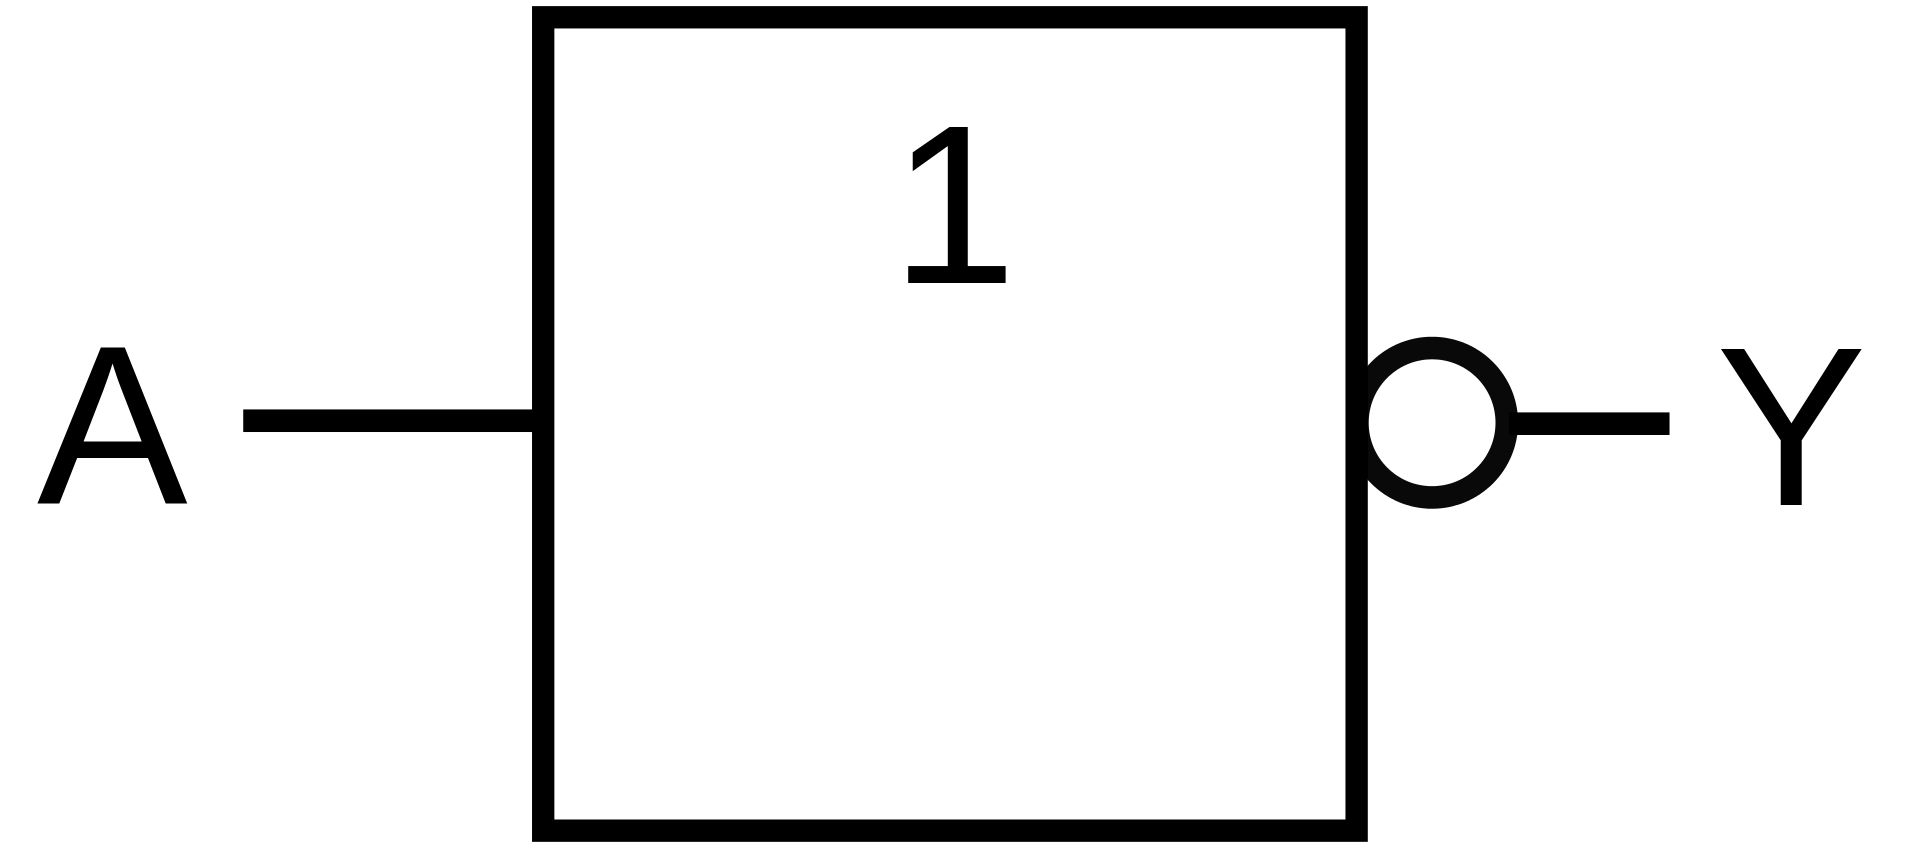
\includegraphics[height = 10mm]{images/not.png}		
        \end{center}
    \end{minipage}
    \hfill
    \begin{minipage}{0.35\linewidth}
        \begin{tabular}{|c|c|}
            \hline
            A & Y\\
            \hline
            0 & 1 \\
            1 & 0 \\
            \hline
        \end{tabular}
    \end{minipage}
\end{center}

\subsubsection{AND}
\begin{center}
	\begin{minipage}{0.55\linewidth}
		$Y = A \land B$ \\
		Y = A\&B
	\begin{center}
		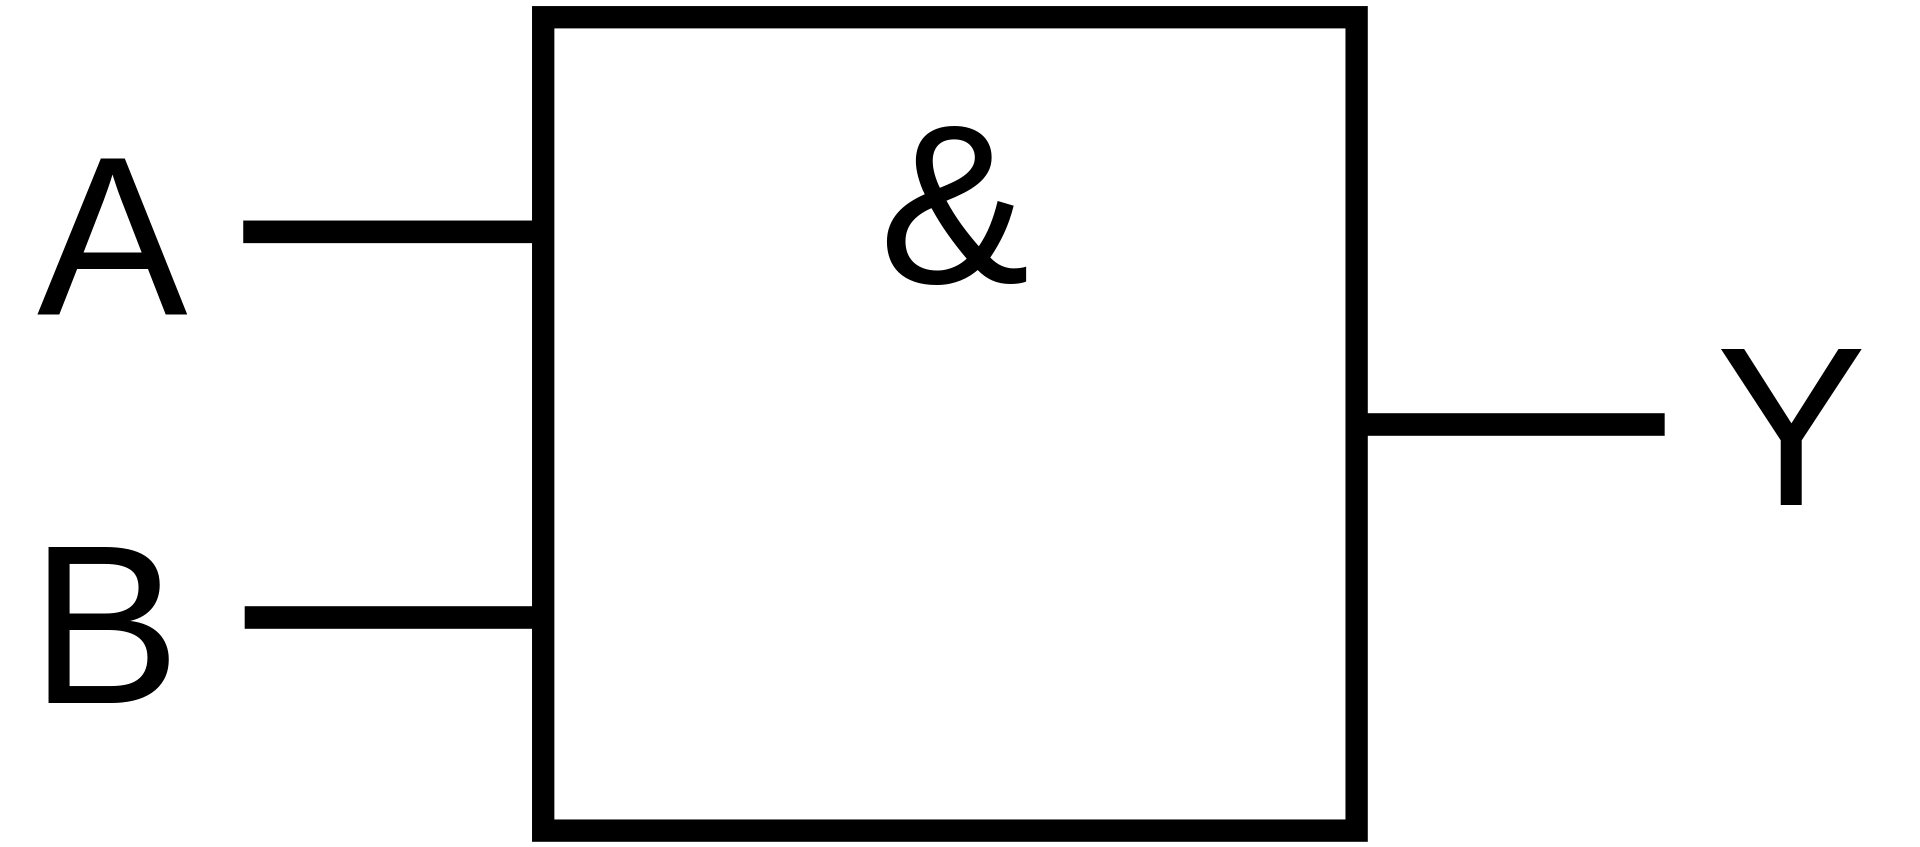
\includegraphics[height = 10mm]{images/and.png}
	\end{center}
    \end{minipage}
    \hfill
    \begin{minipage}{0.35\linewidth}
        \begin{tabular}{|c c|c|}
            \hline
            A & B & Y\\
            \hline
            0 & 0 & 0\\
            0 & 1 & 0\\
            1 & 0 & 0\\
            1 & 1 & 1\\
            \hline
        \end{tabular}
    \end{minipage}
\end{center}

\subsubsection{OR}
\begin{center}
    \begin{minipage}{0.55\linewidth}
		$Y = A \lor B$ \\
		Y = A\#B
        \begin{center}
		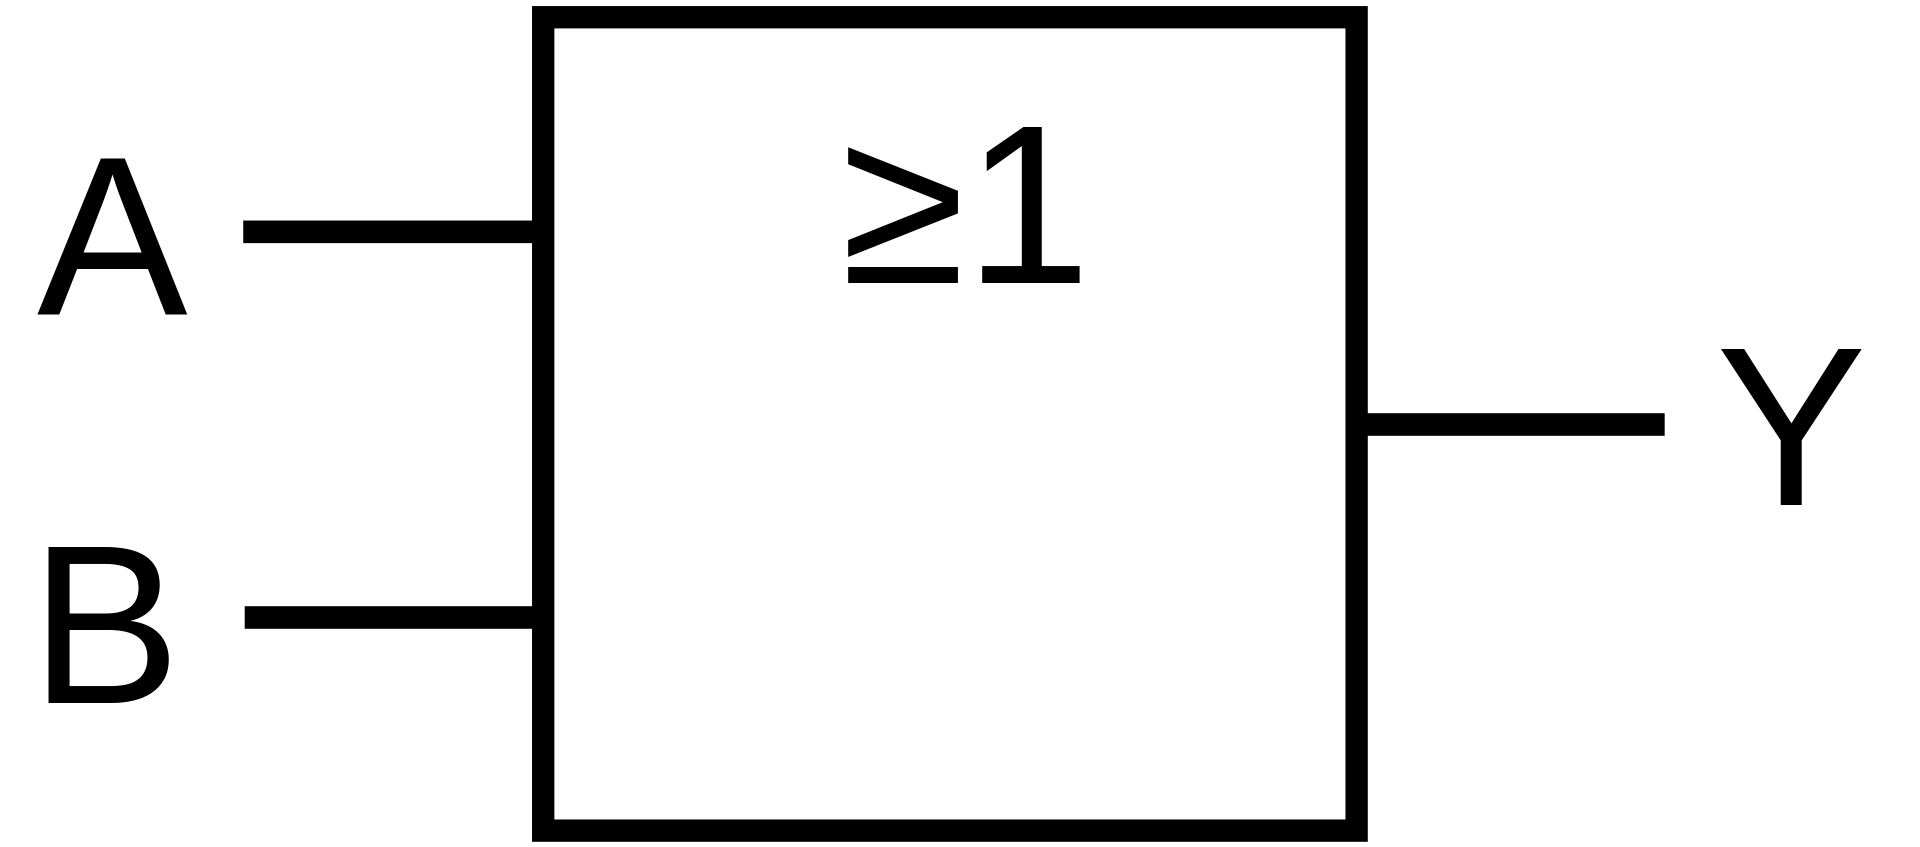
\includegraphics[height = 10mm]{images/or.png}		
        \end{center}
    \end{minipage}
    \hfill
    \begin{minipage}{0.35\linewidth}
        \begin{tabular}{|c c|c|}
            \hline
            A & B & Y\\
            \hline
            0 & 0 & 0\\
            0 & 1 & 1\\
            1 & 0 & 1\\
            1 & 1 & 1\\
            \hline
        \end{tabular}
    \end{minipage}
\end{center}

\subsubsection{EXOR}
\begin{center}
    \begin{minipage}{0.55\linewidth}
		$Y = (A \land \neg B) \lor (\neg A \land B)$ \\
		Y = A \$ B
        \begin{center}
		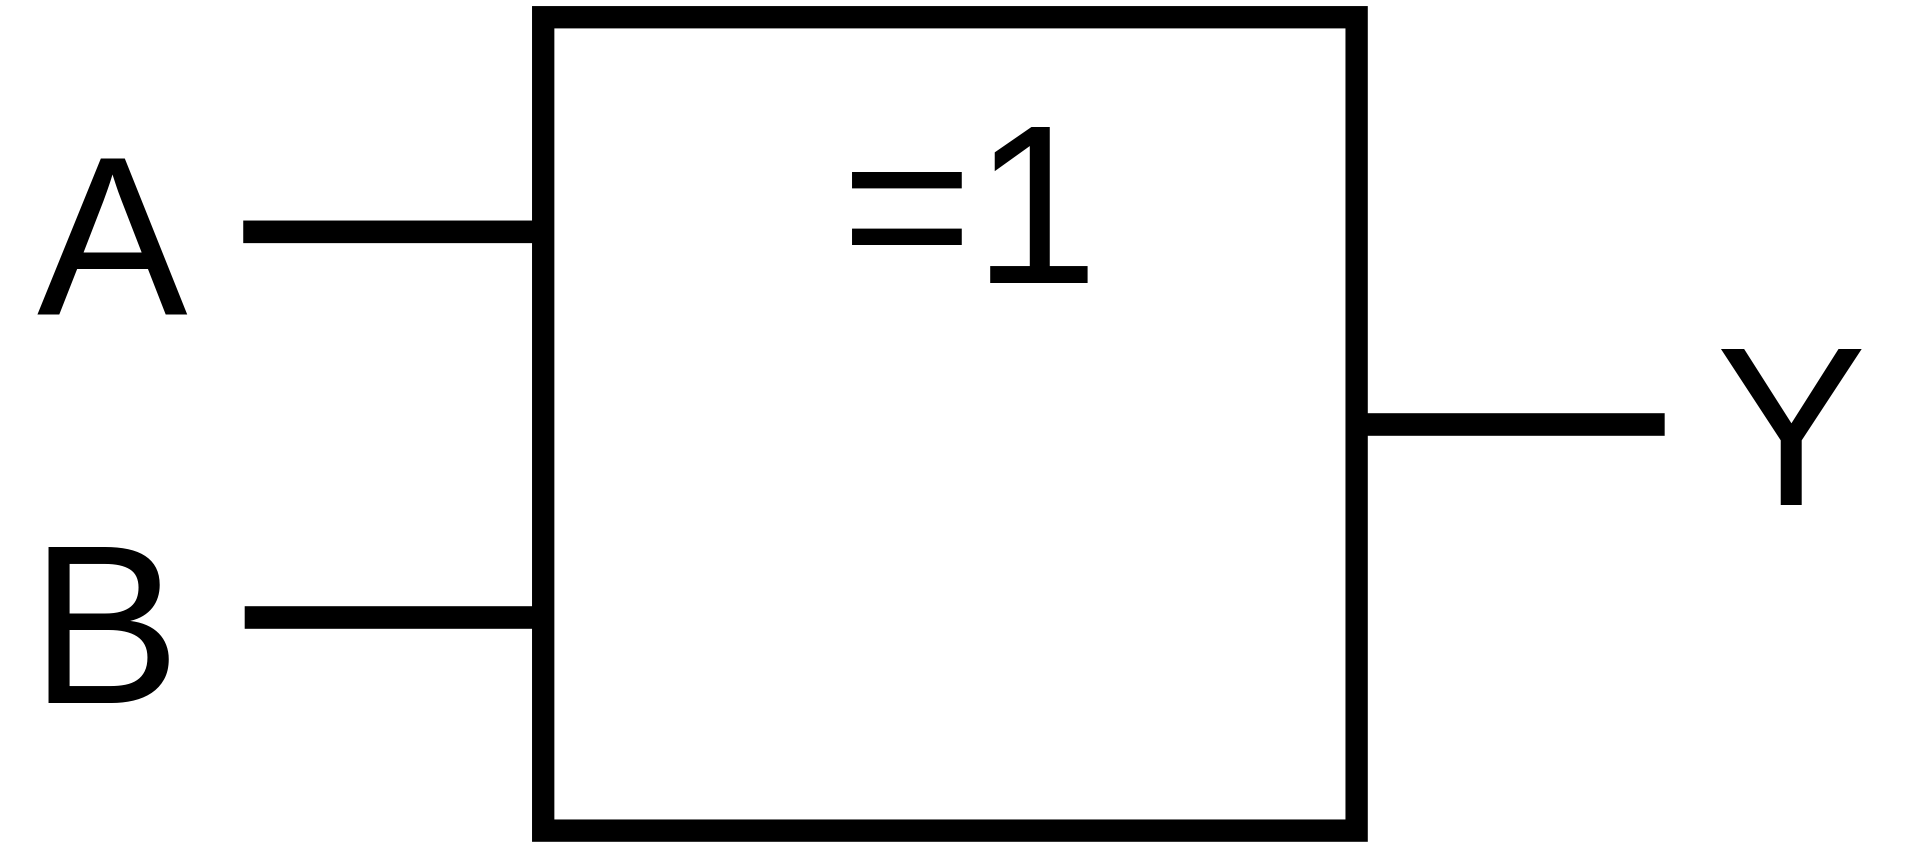
\includegraphics[height = 10mm]{images/xor.png}		
        \end{center}
    \end{minipage}
    \hfill
    \begin{minipage}{0.35\linewidth}
	\begin{tabular}{|c c|c|}
            \hline
            A & B & Y\\
            \hline
            0 & 0 & 0\\
            0 & 1 & 1\\
            1 & 0 & 1\\
	    1 & 1 & 0\\
            \hline
  	  \end{tabular}
    \end{minipage}
\end{center}

\subsubsection{EXNOR}
\begin{center}
    \begin{minipage}{0.55\linewidth}
		$Y = (A \land B) \lor (\neg A \land \neg B)$\\
		Y = !(A \$ B)
        \begin{center}
		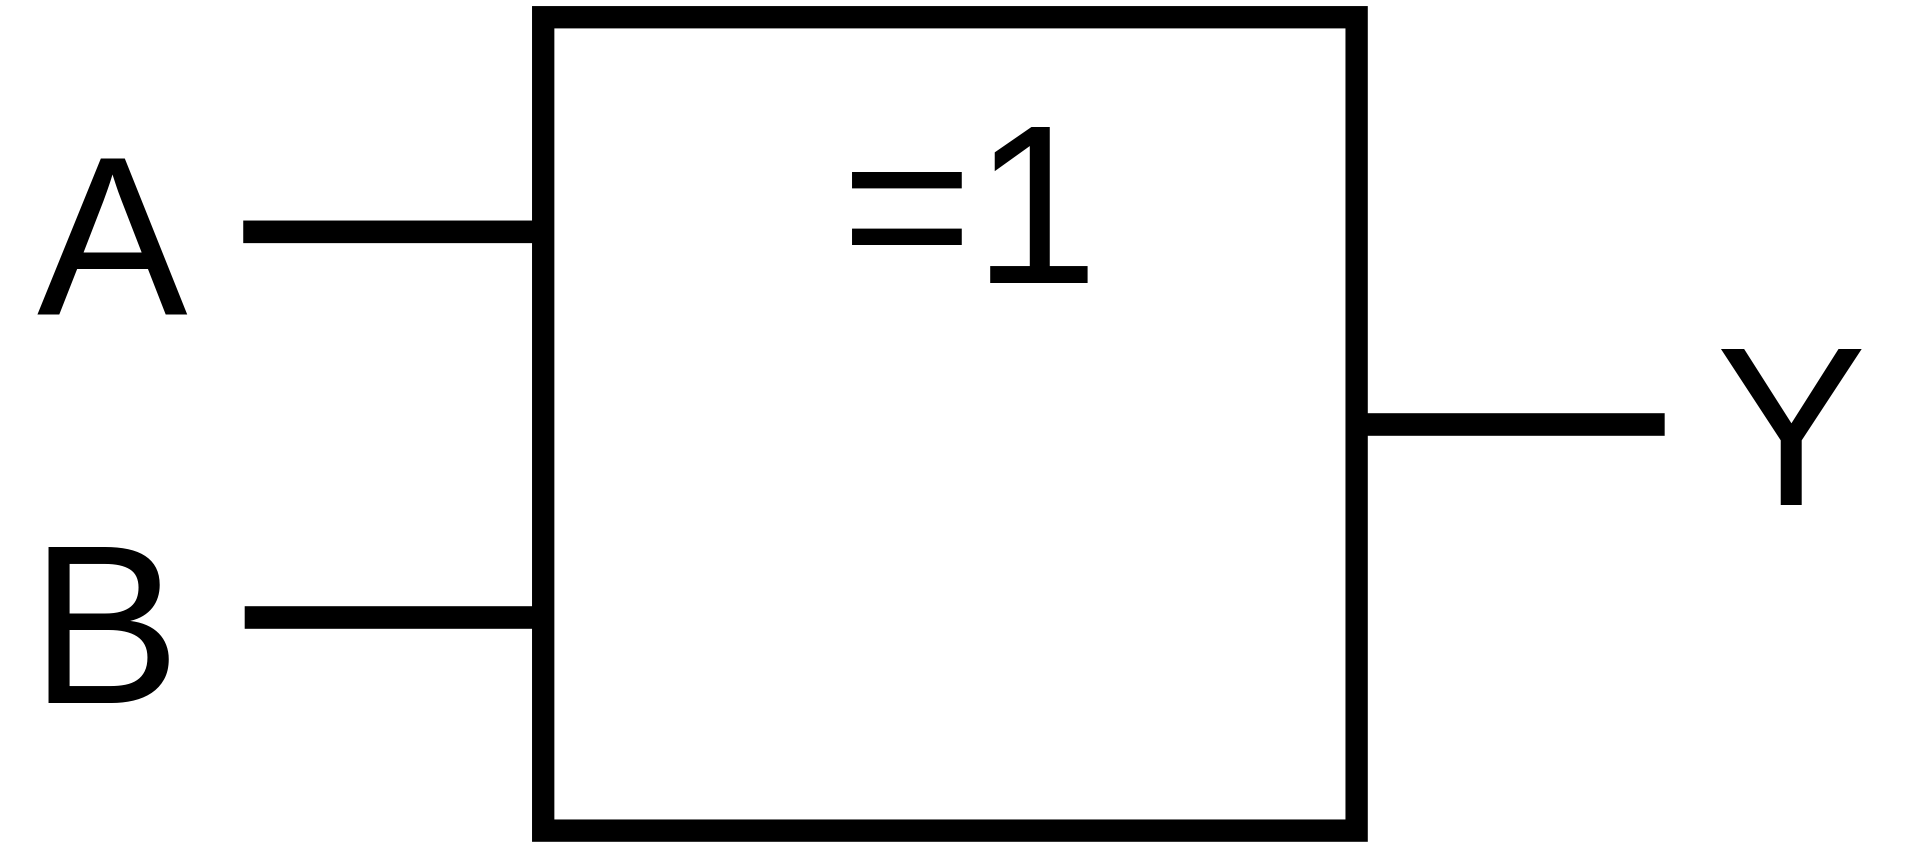
\includegraphics[height = 10mm]{images/xor.png}		
        \end{center}
    \end{minipage}
    \hfill
    \begin{minipage}{0.35\linewidth}
	\begin{tabular}{|c c|c|}
            \hline
            A & B & Y\\
            \hline
            0 & 0 & 0\\
            0 & 1 & 0\\
            1 & 0 & 0\\
	    1 & 1 & 1\\
            \hline
  	  \end{tabular}
    \end{minipage}
\end{center}

\subsubsection{NAND}
\begin{center}
    \begin{minipage}{0.55\linewidth}
		$Y = \neg(A \land B)$\\
		Y = !(A \& B)
        \begin{center}
		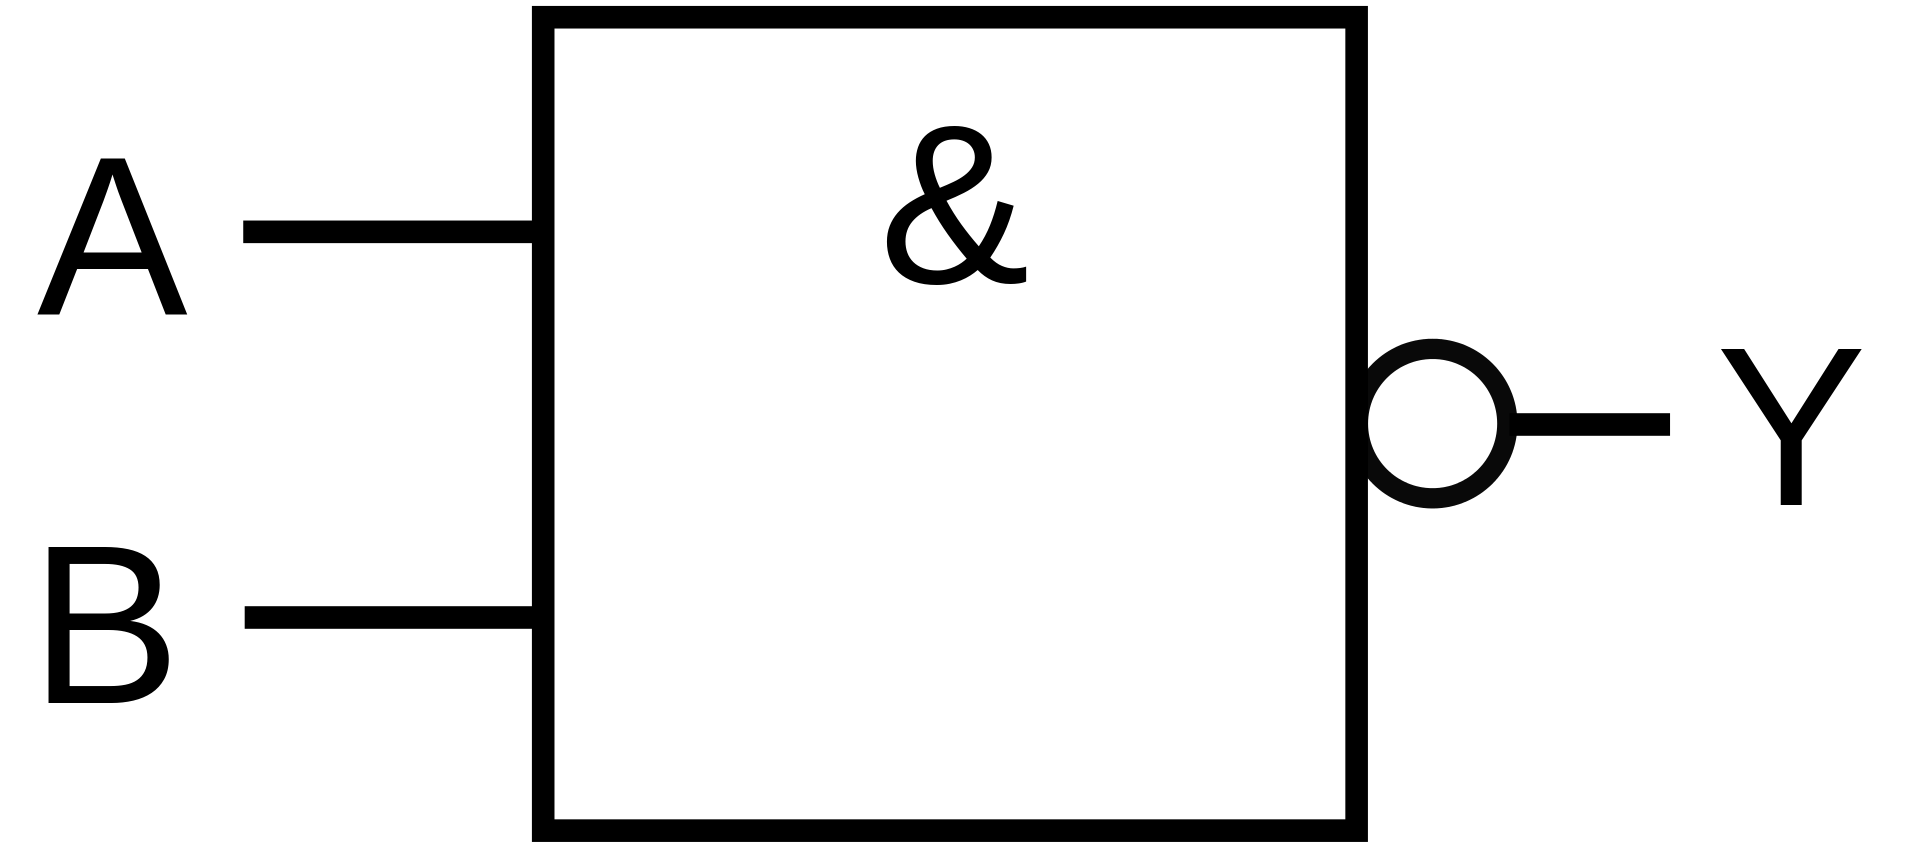
\includegraphics[height = 10mm]{images/nand.png}		
        \end{center}
    \end{minipage}
    \hfill
    \begin{minipage}{0.35\linewidth}
	\begin{tabular}{|c c|c|}
            \hline
            A & B & Y\\
            \hline
            0 & 0 & 1\\
            0 & 1 & 1\\
            1 & 0 & 1\\
	    1 & 1 & 0\\
            \hline
  	  \end{tabular}
    \end{minipage}
\end{center}

\subsubsection{NOR}
\begin{center}
    \begin{minipage}{0.55\linewidth}
		$Y = \neg(A \lor B)$\\
		Y = !(A \# B)
        \begin{center}
		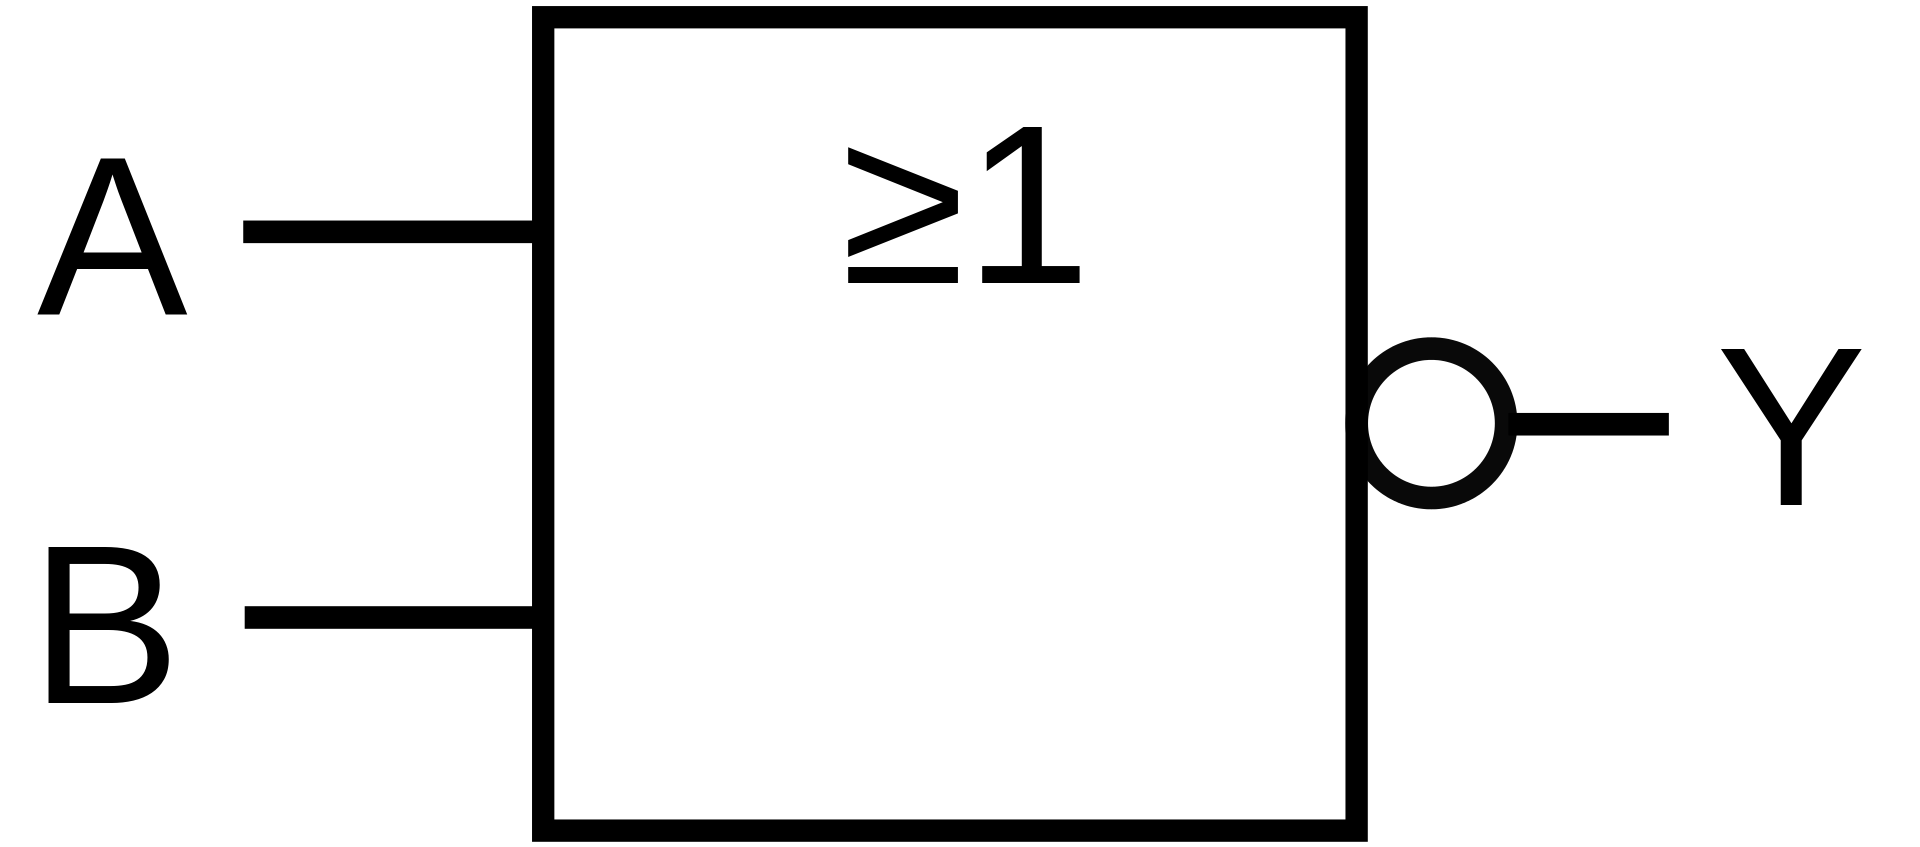
\includegraphics[height = 10mm]{images/nor.png}		
        \end{center}
    \end{minipage}
    \hfill
    \begin{minipage}{0.35\linewidth}
	\begin{tabular}{|c c|c|}
            \hline
            A & B & Y\\
            \hline
            0 & 0 & 1\\
            0 & 1 & 0\\
            1 & 0 & 0\\
	    1 & 1 & 0\\
            \hline
  	  \end{tabular}
    \end{minipage}
\end{center}

\subsection{Vereinfachung boolescher Funktionen}
	Die Disjunktive Normalform DNF besteht ausschliesslich aus OR-Verknüpfungen 
	von AND-verknüpften Eingangsvariabeln. Beispiel: \\
	Z = (A \& B \& C \& D) \# (A \& B \& !C \& !D) \# \\
	(C \& !D) \\
	Jede boolesche Funktion besitzt genau eine DNF.

\subsection{Gesetz von de Morgan}
Das Gesetz von de Morgan besagt:
\begin{itemize}
	\item !(A \& B) = !A \# !B
	\item !(A \# B) = !A \& !B 
\end{itemize}
\subsection{1-Bit Halb Addierer}
Addition von zwei 1-Bit Inputs. \\
\begin{minipage}{1\linewidth}
	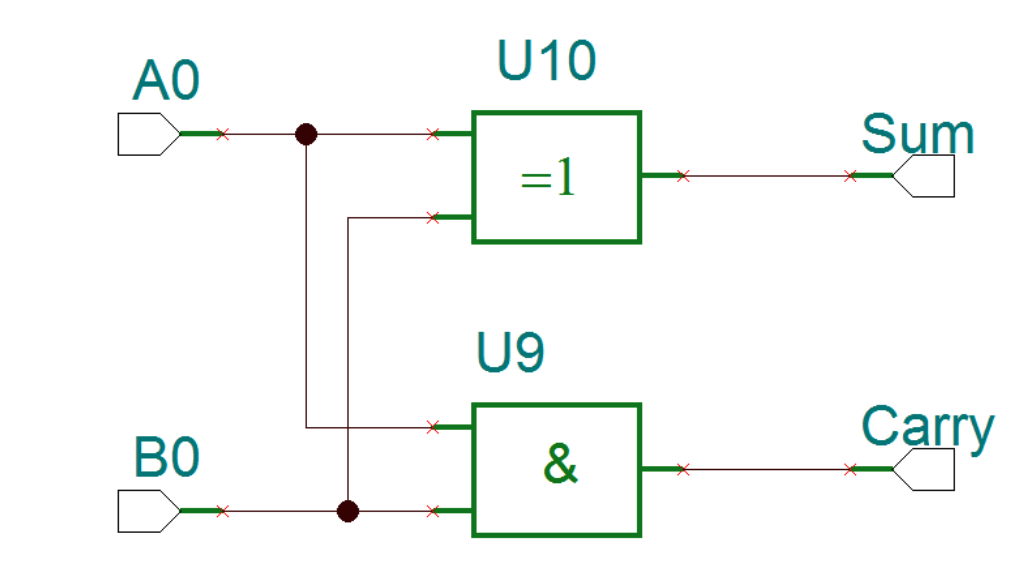
\includegraphics[height=30mm]{images/1bitadd.png}
\end{minipage}
\hfill
\\
\\
\begin{minipage}{1\linewidth}
	\begin{tabular}{| c | c | c | c|}
		\hline
		A0 & B0 & Sum & Carry \\
		\hline
		0 & 0 & 0 & 0 \\
		0 & 1 & 1 & 0 \\
		1 & 0 & 1 & 0 \\
		1 & 1 & 0 & 1 \\
		\hline
	\end{tabular} \\
\end{minipage}
\\
\\
\begin{minipage}{0.55\linewidth}
	\begin{tabular}{c c c c c c}
		  & 0 & 1 & 1 & 1 & \\
		+ & 0 & 1 & 0 & 1 & \\
		0 & 1 & 1 & 1 &   & Carry \\
		\hline
		0 & 1 & 1 & 0 & 0 & Sum \\
	\end{tabular} \\
\end{minipage}
\hfill
\begin{minipage}{0.35\linewidth}
	Sum = A0 \$ B0 \\
	Carry = A0 \& B0
\end{minipage}

\subsection{1-Bit Voll Addierer}
Addition mit Carry In. \\
\begin{minipage}{1\linewidth}
	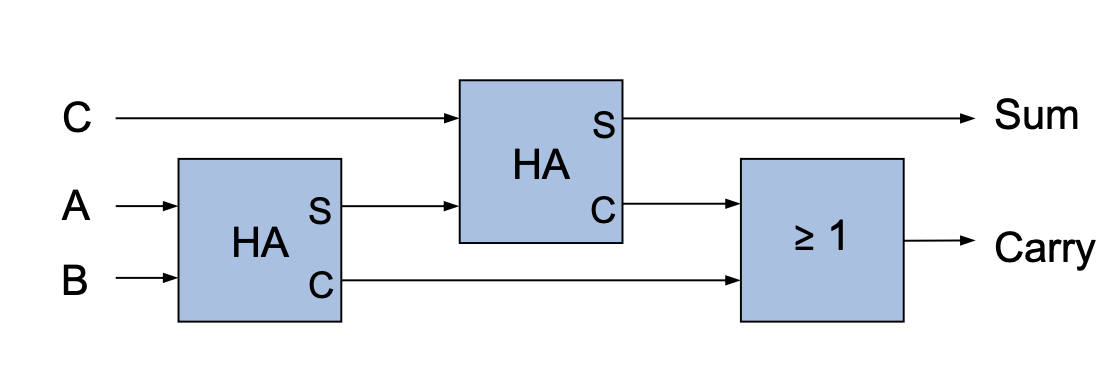
\includegraphics[height=20mm]{images/1bitvoll.png}
\end{minipage}
\hfill
\\
\\
\begin{minipage}{1\linewidth}
	\begin{tabular}{| c | c | c || c| c |}
		\hline
		C & A & B & Sum & Carry \\
		\hline
		0 & 0 & 0 & 0 & 0 \\
		0 & 0 & 1 & 1 & 0 \\
		0 & 1 & 0 & 1 & 0 \\
		0 & 1 & 1 & 0 & 1 \\
		1 & 0 & 0 & 1 & 0 \\
		1 & 0 & 1 & 0 & 1 \\
		1 & 1 & 0 & 0 & 1 \\
		1 & 1 & 1 & 1 & 1 \\
		\hline
	\end{tabular} \\
\end{minipage}


\subsection{4-Bit Addierer}
\begin{minipage}{1\linewidth}
	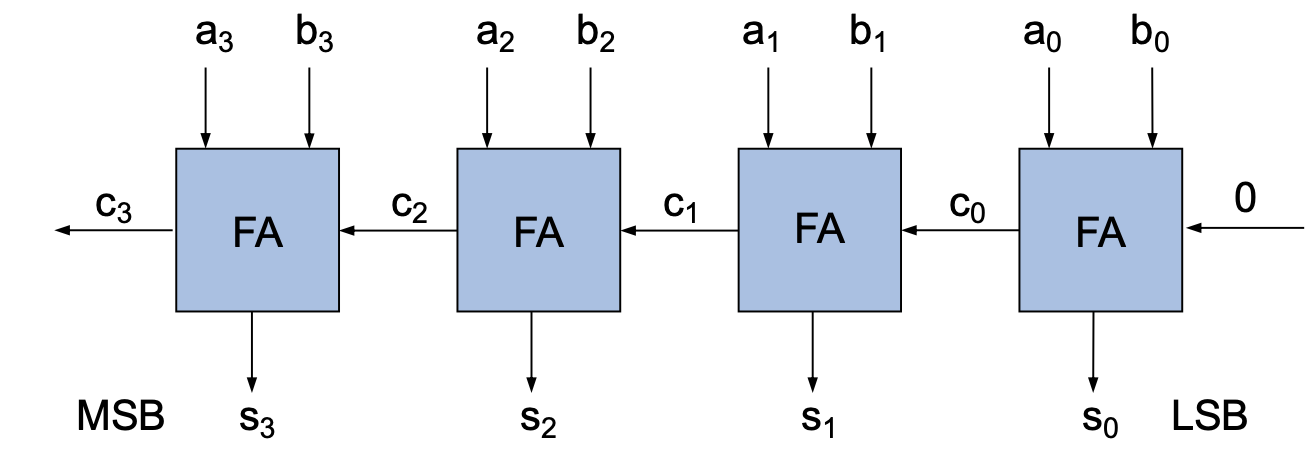
\includegraphics[height=20mm]{images/4bitadd.png}
\end{minipage}
\hfill
\\
\\
\begin{minipage}{1\linewidth}
	\begin{tabular}{| c | c | c || c| c |}
		\hline
		$C_i-1$ & $A_i$ & $B_i$ & $S_i$ & $C_i$ \\
		\hline
		0 & 0 & 0 & 0 & 0 \\
		0 & 0 & 1 & 1 & 0 \\
		0 & 1 & 0 & 1 & 0 \\
		0 & 1 & 1 & 0 & 1 \\
		1 & 0 & 0 & 1 & 0 \\
		1 & 0 & 1 & 0 & 1 \\
		1 & 1 & 0 & 0 & 1 \\
		1 & 1 & 1 & 1 & 1 \\
		\hline
	\end{tabular} \\
\end{minipage}

